\documentclass[aspectratio=169, 11pt]{beamer}

% Theme matching the existing slides
\usetheme{Madrid}
\usecolortheme{whale}

% Custom colors to match existing slides
\definecolor{dgistnavy}{RGB}{0,51,102}
\definecolor{dgistlight}{RGB}{220,230,240}
\definecolor{dgistgreen}{RGB}{0,128,100}
\definecolor{dgistred}{RGB}{180,40,40}

\setbeamercolor{structure}{fg=dgistnavy}
\setbeamercolor{frametitle}{bg=dgistnavy, fg=white}
\setbeamercolor{title}{bg=dgistnavy, fg=white}
\setbeamercolor{block title}{bg=dgistnavy, fg=white}
\setbeamercolor{block body}{bg=dgistlight, fg=black}
\setbeamercolor{block title example}{bg=dgistgreen, fg=white}
\setbeamercolor{block body example}{bg=green!5, fg=black}
\setbeamercolor{block title alerted}{bg=dgistred, fg=white}
\setbeamercolor{block body alerted}{bg=red!5, fg=black}

\setbeamertemplate{navigation symbols}{}
\setbeamertemplate{footline}{%
  \leavevmode%
  \hbox{%
  \begin{beamercolorbox}[wd=.333333\paperwidth,ht=2.25ex,dp=1ex,center]{author in head/foot}%
    \usebeamerfont{author in head/foot}DGIST RT604 SLAM
  \end{beamercolorbox}%
  \begin{beamercolorbox}[wd=.333333\paperwidth,ht=2.25ex,dp=1ex,center]{title in head/foot}%
    \usebeamerfont{title in head/foot}Gaussian Linear Transformation Recap
  \end{beamercolorbox}%
  \begin{beamercolorbox}[wd=.333333\paperwidth,ht=2.25ex,dp=1ex,right]{date in head/foot}%
    \usebeamerfont{date in head/foot}%
    \insertframenumber{}/\inserttotalframenumber\hspace*{2ex}
  \end{beamercolorbox}}%
  \vskip0pt%
}

\usepackage{amsmath,amssymb,bm}
\usepackage{tikz}
\usetikzlibrary{arrows.meta, positioning, calc, decorations.pathreplacing}

\newcommand{\E}{\mathbb{E}}
\newcommand{\Var}{\mathrm{Var}}
\newcommand{\Cov}{\mathrm{Cov}}
\newcommand{\T}{^{\top}}

\title{Recap: Linear Transformation of Gaussians}
\subtitle{From Probability Theory to Odometry Covariance Propagation}
\institute{RT604 SLAM Course\\Department of Robotics \& Mechatronics Engineering\\DGIST}
\date{Spring 2026}

\begin{document}

% ==================== TITLE ====================
{
\setbeamertemplate{footline}{}
\begin{frame}
\titlepage
\end{frame}
}

% ==================== OUTLINE ====================
\begin{frame}{Outline}
\begin{enumerate}
  \setlength{\itemsep}{12pt}
  \item Review: Mean and Covariance
  \item Affine Transformation: $\mathbf{y} = \mathbf{A}\mathbf{x} + \mathbf{b}$
  \item Derivation of Transformed Mean and Covariance
  \item Generalization: $\mathbf{y} = \sum_i \mathbf{A}_i \mathbf{x}_i + \mathbf{b}$
  \item Connection to Odometry Covariance Propagation
\end{enumerate}
\end{frame}

% ==================== REVIEW: MEAN AND COV ====================
\begin{frame}{Review: Mean and Covariance}

\begin{block}{Mean (Expected Value)}
$$\bm{\mu}_{\mathbf{x}} = \E[\mathbf{x}] = \int \mathbf{x} \, p(\mathbf{x}) \, d\mathbf{x}$$
\end{block}

\vspace{4pt}

\begin{block}{Covariance Matrix}
$$\bm{\Sigma}_{\mathbf{x}} = \E\!\left[(\mathbf{x} - \bm{\mu}_{\mathbf{x}})(\mathbf{x} - \bm{\mu}_{\mathbf{x}})\T\right]$$
\end{block}

\vspace{6pt}

Key properties we will use:
\begin{itemize}
  \item Linearity of expectation: $\E[\mathbf{A}\mathbf{x} + \mathbf{b}] = \mathbf{A}\,\E[\mathbf{x}] + \mathbf{b}$
  \item Constants factor out: $\E[\mathbf{A}\mathbf{x}] = \mathbf{A}\,\E[\mathbf{x}]$ (works for any matrix $\mathbf{A}$)
\end{itemize}

\end{frame}

% ==================== GAUSSIAN REMINDER ====================
\begin{frame}{Gaussian (Normal) Distribution}

A random vector $\mathbf{x} \in \mathbb{R}^n$ is \textbf{Gaussian} if:
$$\mathbf{x} \sim \mathcal{N}(\bm{\mu}, \bm{\Sigma})$$

\vspace{-4pt}
with probability density:
$$p(\mathbf{x}) = \frac{1}{\sqrt{(2\pi)^n \det(\bm{\Sigma})}} \exp\!\left(-\tfrac{1}{2}(\mathbf{x}-\bm{\mu})\T \bm{\Sigma}^{-1}(\mathbf{x}-\bm{\mu})\right)$$

\vspace{8pt}

\begin{alertblock}{Key Property}
A Gaussian distribution is \textbf{completely characterized} by just two parameters:
$$\bm{\mu} \quad \text{(mean vector)} \qquad \bm{\Sigma} \quad \text{(covariance matrix)}$$
So if we can compute the mean and covariance of a transformed variable, we know its entire distribution.
\end{alertblock}

\end{frame}

% ==================== AFFINE TRANSFORMATION: STATEMENT ====================
\begin{frame}{Affine Transformation of a Gaussian}

\begin{block}{The Setup}
Given: $\mathbf{x} \sim \mathcal{N}(\bm{\mu}_{\mathbf{x}},\; \bm{\Sigma}_{\mathbf{x}})$, \quad
a constant matrix $\mathbf{A}$, \quad
a constant vector $\mathbf{b}$.

\vspace{6pt}
Define a new random variable:
$$\mathbf{y} = \mathbf{A}\mathbf{x} + \mathbf{b}$$
\end{block}

\vspace{6pt}

\begin{exampleblock}{Result}
$$\mathbf{y} \sim \mathcal{N}\!\left(\mathbf{A}\bm{\mu}_{\mathbf{x}} + \mathbf{b},\;\; \mathbf{A}\,\bm{\Sigma}_{\mathbf{x}}\,\mathbf{A}\T\right)$$
\end{exampleblock}

\vspace{6pt}

That is:
\begin{itemize}
  \item $\bm{\mu}_{\mathbf{y}} = \mathbf{A}\bm{\mu}_{\mathbf{x}} + \mathbf{b}$
  \item $\bm{\Sigma}_{\mathbf{y}} = \mathbf{A}\,\bm{\Sigma}_{\mathbf{x}}\,\mathbf{A}\T$
\end{itemize}

\end{frame}

% ==================== DERIVATION: MEAN ====================
\begin{frame}{Derivation: Mean of $\mathbf{y} = \mathbf{A}\mathbf{x} + \mathbf{b}$}

\begin{block}{Step-by-step}
\begin{align*}
\bm{\mu}_{\mathbf{y}} &= \E[\mathbf{y}] \\[6pt]
&= \E[\mathbf{A}\mathbf{x} + \mathbf{b}] \\[6pt]
&= \E[\mathbf{A}\mathbf{x}] + \E[\mathbf{b}]
  \qquad \text{\small (linearity of expectation)} \\[6pt]
&= \mathbf{A}\,\E[\mathbf{x}] + \mathbf{b}
  \qquad \text{\small ($\mathbf{A}$ is constant, $\mathbf{b}$ is constant)} \\[6pt]
&= \boxed{\mathbf{A}\bm{\mu}_{\mathbf{x}} + \mathbf{b}}
\end{align*}
\end{block}

\vspace{6pt}
Intuition: the mean transforms in exactly the same way as the variable itself.

\end{frame}

% ==================== DERIVATION: COVARIANCE ====================
\begin{frame}{Derivation: Covariance of $\mathbf{y} = \mathbf{A}\mathbf{x} + \mathbf{b}$}

\begin{block}{Step-by-step}
\begin{align*}
\bm{\Sigma}_{\mathbf{y}}
  &= \E\!\left[(\mathbf{y} - \bm{\mu}_{\mathbf{y}})(\mathbf{y} - \bm{\mu}_{\mathbf{y}})\T\right] \\[6pt]
  &= \E\!\left[\bigl((\mathbf{A}\mathbf{x}+\mathbf{b}) - (\mathbf{A}\bm{\mu}_{\mathbf{x}}+\mathbf{b})\bigr)
    \bigl((\mathbf{A}\mathbf{x}+\mathbf{b}) - (\mathbf{A}\bm{\mu}_{\mathbf{x}}+\mathbf{b})\bigr)\T\right] \\[6pt]
  &= \E\!\left[\mathbf{A}(\mathbf{x} - \bm{\mu}_{\mathbf{x}})
    \bigl(\mathbf{A}(\mathbf{x}-\bm{\mu}_{\mathbf{x}})\bigr)\T\right]
    \qquad \text{\small ($\mathbf{b}$ cancels!)} \\[6pt]
  &= \E\!\left[\mathbf{A}(\mathbf{x}-\bm{\mu}_{\mathbf{x}})
    (\mathbf{x}-\bm{\mu}_{\mathbf{x}})\T \mathbf{A}\T\right]
    \qquad \text{\small (transpose rule)} \\[6pt]
  &= \mathbf{A}\,\E\!\left[(\mathbf{x}-\bm{\mu}_{\mathbf{x}})
    (\mathbf{x}-\bm{\mu}_{\mathbf{x}})\T\right]\mathbf{A}\T
    \qquad \text{\small ($\mathbf{A}$ is constant)} \\[6pt]
  &= \boxed{\mathbf{A}\,\bm{\Sigma}_{\mathbf{x}}\,\mathbf{A}\T}
\end{align*}
\end{block}

\end{frame}

% ==================== KEY OBSERVATION ====================
\begin{frame}{Key Observations}

\begin{columns}[T]
\begin{column}{0.48\textwidth}
\begin{alertblock}{The bias $\mathbf{b}$ does NOT affect covariance}
$$\bm{\Sigma}_{\mathbf{y}} = \mathbf{A}\,\bm{\Sigma}_{\mathbf{x}}\,\mathbf{A}\T$$
The $\mathbf{b}$ term shifts the mean but does not change the ``spread'' of the distribution.
\end{alertblock}
\end{column}
\begin{column}{0.48\textwidth}
\begin{exampleblock}{Gaussian in $\Rightarrow$ Gaussian out}
A linear (affine) transformation of a Gaussian random variable is still Gaussian.

\vspace{4pt}
This is \textbf{not} true for general nonlinear transformations!
(That is why we need linearization / Jacobians later.)
\end{exampleblock}
\end{column}
\end{columns}

\vspace{10pt}

\begin{center}
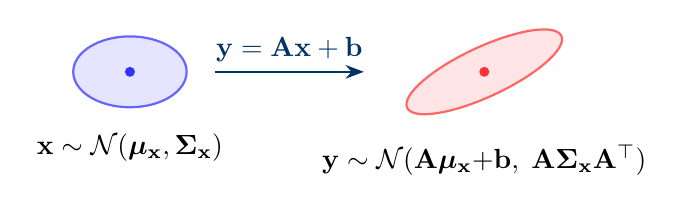
\begin{tikzpicture}[>=Stealth, scale=0.9]
  % Input
  \draw[thick, blue!60, fill=blue!10] (0,0) ellipse (0.8 and 0.5);
  \fill[blue!80] (0,0) circle (2pt);
  \node[below=6pt] at (0,-0.5) {$\mathbf{x} \sim \mathcal{N}(\bm{\mu}_{\mathbf{x}}, \bm{\Sigma}_{\mathbf{x}})$};

  % Arrow
  \draw[->, thick, dgistnavy] (1.2,0) -- (3.3,0)
    node[midway, above] {$\mathbf{y}=\mathbf{A}\mathbf{x}+\mathbf{b}$};

  % Output
  \begin{scope}[shift={(5,0)}, rotate=25]
    \draw[thick, red!60, fill=red!10] (0,0) ellipse (1.2 and 0.35);
  \end{scope}
  \fill[red!80] (5,0) circle (2pt);
  \node[below=10pt] at (5,-0.5) {$\mathbf{y} \sim \mathcal{N}(\mathbf{A}\bm{\mu}_{\mathbf{x}}{+}\mathbf{b},\; \mathbf{A}\bm{\Sigma}_{\mathbf{x}}\mathbf{A}\T)$};
\end{tikzpicture}
\end{center}

\end{frame}

% ==================== SIMPLE SCALAR EXAMPLE ====================
\begin{frame}{Quick Sanity Check: Scalar Case}

Let $x \sim \mathcal{N}(\mu, \sigma^2)$ and $y = ax + b$. Then:

\begin{align*}
  \E[y] &= a\mu + b \\[4pt]
  \Var(y) &= a^2 \sigma^2
\end{align*}

\vspace{6pt}

\begin{exampleblock}{Example}
$x \sim \mathcal{N}(0, 1)$, \quad $y = 3x + 5$

\vspace{4pt}
$\Rightarrow\; \E[y] = 3 \cdot 0 + 5 = 5$, \quad $\Var(y) = 3^2 \cdot 1 = 9$

\vspace{4pt}
$\Rightarrow\; y \sim \mathcal{N}(5,\, 9)$
\end{exampleblock}

\vspace{6pt}

This is the 1D version of $\bm{\Sigma}_{\mathbf{y}} = \mathbf{A}\bm{\Sigma}_{\mathbf{x}}\mathbf{A}\T$.

\vspace{2pt}
In 1D: $\sigma_y^2 = a \cdot \sigma_x^2 \cdot a = a^2 \sigma_x^2$. \; ($a\T = a$ for scalars.)

\end{frame}

% ==================== GENERALIZATION: TWO INDEPENDENT INPUTS ====================
\begin{frame}{Generalization: Sum of Two Independent Terms}

Now suppose $\mathbf{x}_1$ and $\mathbf{x}_2$ are \textbf{independent} random vectors:

\begin{block}{Linear Combination of Two Independent Variables}
$$\mathbf{y} = \mathbf{A}_1 \mathbf{x}_1 + \mathbf{A}_2 \mathbf{x}_2 + \mathbf{b}$$
\end{block}

\vspace{4pt}

\textbf{Mean:}
$$\bm{\mu}_{\mathbf{y}} = \mathbf{A}_1 \bm{\mu}_{\mathbf{x}_1} + \mathbf{A}_2 \bm{\mu}_{\mathbf{x}_2} + \mathbf{b}$$

\vspace{4pt}

\textbf{Covariance:}
$$\boxed{\bm{\Sigma}_{\mathbf{y}}
  = \mathbf{A}_1 \bm{\Sigma}_{\mathbf{x}_1} \mathbf{A}_1\T
  + \mathbf{A}_2 \bm{\Sigma}_{\mathbf{x}_2} \mathbf{A}_2\T}$$

\vspace{8pt}
The covariance contributions from $\mathbf{x}_1$ and $\mathbf{x}_2$ simply \textbf{add up}
because independence means the cross-covariance is zero:
$\Cov(\mathbf{x}_1, \mathbf{x}_2) = \mathbf{0}$.

\end{frame}

% ==================== DERIVATION: TWO INDEPENDENT ====================
\begin{frame}{Derivation: Why Covariances Add for Independent Variables}

Let $\mathbf{y} = \mathbf{A}_1 \mathbf{x}_1 + \mathbf{A}_2 \mathbf{x}_2 + \mathbf{b}$ with $\mathbf{x}_1 \perp \mathbf{x}_2$ (independent).

\vspace{4pt}

Define deviations: $\tilde{\mathbf{x}}_i = \mathbf{x}_i - \bm{\mu}_{\mathbf{x}_i}$, \; then $\mathbf{y} - \bm{\mu}_{\mathbf{y}} = \mathbf{A}_1 \tilde{\mathbf{x}}_1 + \mathbf{A}_2 \tilde{\mathbf{x}}_2$.

\begin{align*}
\bm{\Sigma}_{\mathbf{y}}
  &= \E\!\left[(\mathbf{A}_1 \tilde{\mathbf{x}}_1 + \mathbf{A}_2 \tilde{\mathbf{x}}_2)
    (\mathbf{A}_1 \tilde{\mathbf{x}}_1 + \mathbf{A}_2 \tilde{\mathbf{x}}_2)\T\right] \\[6pt]
  &= \E\!\left[
    \mathbf{A}_1 \tilde{\mathbf{x}}_1 \tilde{\mathbf{x}}_1\T \mathbf{A}_1\T
    + \mathbf{A}_1 \tilde{\mathbf{x}}_1 \tilde{\mathbf{x}}_2\T \mathbf{A}_2\T
    + \mathbf{A}_2 \tilde{\mathbf{x}}_2 \tilde{\mathbf{x}}_1\T \mathbf{A}_1\T
    + \mathbf{A}_2 \tilde{\mathbf{x}}_2 \tilde{\mathbf{x}}_2\T \mathbf{A}_2\T
    \right] \\[6pt]
  &= \mathbf{A}_1 \underbrace{\E[\tilde{\mathbf{x}}_1\tilde{\mathbf{x}}_1\T]}_{\bm{\Sigma}_{\mathbf{x}_1}} \mathbf{A}_1\T
    + \mathbf{A}_1 \underbrace{\E[\tilde{\mathbf{x}}_1\tilde{\mathbf{x}}_2\T]}_{\mathbf{0}\;\text{(indep.)}} \mathbf{A}_2\T
    + \mathbf{A}_2 \underbrace{\E[\tilde{\mathbf{x}}_2\tilde{\mathbf{x}}_1\T]}_{\mathbf{0}\;\text{(indep.)}} \mathbf{A}_1\T
    + \mathbf{A}_2 \underbrace{\E[\tilde{\mathbf{x}}_2\tilde{\mathbf{x}}_2\T]}_{\bm{\Sigma}_{\mathbf{x}_2}} \mathbf{A}_2\T
\end{align*}

$$= \boxed{\mathbf{A}_1 \bm{\Sigma}_{\mathbf{x}_1} \mathbf{A}_1\T + \mathbf{A}_2 \bm{\Sigma}_{\mathbf{x}_2} \mathbf{A}_2\T}$$

\end{frame}

% ==================== GENERAL CASE ====================
\begin{frame}{General Case: $N$ Independent Inputs}

\begin{block}{General Linear Combination}
$$\mathbf{y} = \sum_{i=1}^{N} \mathbf{A}_i \mathbf{x}_i + \mathbf{b}, \qquad \mathbf{x}_i \perp \mathbf{x}_j \;\;\forall\; i \neq j$$
\end{block}

\vspace{6pt}

\textbf{Mean:}
$$\bm{\mu}_{\mathbf{y}} = \sum_{i=1}^{N} \mathbf{A}_i \bm{\mu}_{\mathbf{x}_i} + \mathbf{b}$$

\vspace{4pt}

\textbf{Covariance:}
$$\boxed{\bm{\Sigma}_{\mathbf{y}} = \sum_{i=1}^{N} \mathbf{A}_i \bm{\Sigma}_{\mathbf{x}_i} \mathbf{A}_i\T}$$

\vspace{6pt}

Each independent noise source contributes its own $\mathbf{A}_i \bm{\Sigma}_{\mathbf{x}_i} \mathbf{A}_i\T$ term.

The total covariance is the sum of all these contributions.

\end{frame}

% ==================== CONNECTION TO ODOMETRY ====================
\begin{frame}{Connection to Odometry Covariance Propagation}

Recall the odometry update is a \textbf{nonlinear} function of two independent inputs:

$$\mathbf{p}' = f\!\left(\mathbf{p},\; \Delta \mathbf{r}\right),
\qquad \Delta\mathbf{r} = \begin{pmatrix}\Delta s_R \\ \Delta s_L\end{pmatrix}$$

\vspace{4pt}

After \textbf{first-order linearization} (Taylor expansion):

$$\mathbf{p}' \approx f(\hat{\mathbf{p}}, \hat{\Delta\mathbf{r}})
  + \underbrace{\frac{\partial f}{\partial \mathbf{p}}}_{\mathbf{F}_\mathbf{p}} (\mathbf{p} - \hat{\mathbf{p}})
  + \underbrace{\frac{\partial f}{\partial \Delta\mathbf{r}}}_{\mathbf{F}_\Delta} (\Delta\mathbf{r} - \hat{\Delta\mathbf{r}})$$

\vspace{6pt}

This is exactly in the form $\mathbf{y} = \mathbf{A}_1 \mathbf{x}_1 + \mathbf{A}_2 \mathbf{x}_2 + \mathbf{b}$ with:

\begin{center}
\renewcommand{\arraystretch}{1.4}
\begin{tabular}{c|c|c}
  & Variable $\mathbf{x}_i$ & Matrix $\mathbf{A}_i$ \\
  \hline
  Source 1 & $\mathbf{p} - \hat{\mathbf{p}}$ (prior pose error) & $\mathbf{F}_\mathbf{p}$ (Jacobian w.r.t.\ pose) \\
  Source 2 & $\Delta\mathbf{r} - \hat{\Delta\mathbf{r}}$ (wheel noise) & $\mathbf{F}_\Delta$ (Jacobian w.r.t.\ wheels) \\
\end{tabular}
\end{center}

\end{frame}

% ==================== THE EQUATION ====================
\begin{frame}{Applying the Rule: Odometry Covariance}

Applying the linear combination covariance formula directly:

$$\bm{\Sigma}_{\mathbf{y}} = \mathbf{A}_1 \bm{\Sigma}_{\mathbf{x}_1} \mathbf{A}_1\T + \mathbf{A}_2 \bm{\Sigma}_{\mathbf{x}_2} \mathbf{A}_2\T$$

\vspace{4pt}

\begin{block}{Odometry Covariance Propagation (Siegwart Eq.\ 5.9)}
$$\boxed{\bm{\Sigma}_{\mathbf{p}'} = \mathbf{F}_\mathbf{p}\, \bm{\Sigma}_{\mathbf{p}}\, \mathbf{F}_\mathbf{p}\T + \mathbf{F}_\Delta\, \bm{\Sigma}_\Delta\, \mathbf{F}_\Delta\T}$$
\end{block}

\vspace{6pt}

\begin{center}
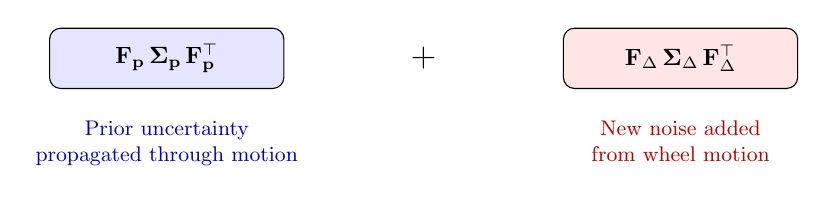
\begin{tikzpicture}[>=Stealth, node distance=1.2cm, scale=0.85, every node/.style={scale=0.85}]
  \node[draw, rounded corners, fill=blue!10, minimum width=3.5cm, minimum height=0.9cm, align=center]
    (term1) {$\mathbf{F}_\mathbf{p}\, \bm{\Sigma}_{\mathbf{p}}\, \mathbf{F}_\mathbf{p}\T$};
  \node[below=0.3cm of term1, text=blue!70!black, align=center, font=\small]
    (label1) {Prior uncertainty\\propagated through motion};

  \node[right=1.5cm of term1, font=\Large] (plus) {$+$};

  \node[right=1.5cm of plus, draw, rounded corners, fill=red!10, minimum width=3.5cm, minimum height=0.9cm, align=center]
    (term2) {$\mathbf{F}_\Delta\, \bm{\Sigma}_\Delta\, \mathbf{F}_\Delta\T$};
  \node[below=0.3cm of term2, text=red!70!black, align=center, font=\small]
    (label2) {New noise added\\from wheel motion};
\end{tikzpicture}
\end{center}

\vspace{4pt}

Both terms have the \textbf{same structure}: $\mathbf{A}\bm{\Sigma}\mathbf{A}\T$.

This is nothing more than the Gaussian linear transformation rule applied twice!

\end{frame}

% ==================== WHY LINEARIZATION ====================
\begin{frame}{Why Do We Need Jacobians?}

The odometry function $f(\mathbf{p}, \Delta\mathbf{r})$ is \textbf{nonlinear} (contains $\sin\theta$, $\cos\theta$).

\vspace{4pt}

The rule $\bm{\Sigma}_{\mathbf{y}} = \mathbf{A}\bm{\Sigma}_{\mathbf{x}}\mathbf{A}\T$ only works for \textbf{linear} transformations.

\vspace{6pt}

\begin{alertblock}{Solution: First-Order Taylor Approximation}
Locally approximate the nonlinear function by a linear one:
$$f(\mathbf{x}) \approx f(\hat{\mathbf{x}}) + \underbrace{\left.\frac{\partial f}{\partial \mathbf{x}}\right|_{\hat{\mathbf{x}}}}_{\text{Jacobian } \mathbf{J}} (\mathbf{x} - \hat{\mathbf{x}})$$

Now the deviation $(\mathbf{x} - \hat{\mathbf{x}})$ is transformed \textbf{linearly} by $\mathbf{J}$.

$\Rightarrow$ We can apply: $\bm{\Sigma}_{\mathbf{y}} \approx \mathbf{J}\,\bm{\Sigma}_{\mathbf{x}}\,\mathbf{J}\T$
\end{alertblock}

\vspace{6pt}

This is the core idea behind the \textbf{Extended Kalman Filter (EKF)}:

use Jacobians to apply linear Gaussian rules to nonlinear systems.

\end{frame}

% ==================== SUMMARY ====================
\begin{frame}{Summary}

\begin{enumerate}
\setlength{\itemsep}{10pt}

\item \textbf{Single affine transformation:} If $\mathbf{y} = \mathbf{A}\mathbf{x} + \mathbf{b}$ and $\mathbf{x} \sim \mathcal{N}(\bm{\mu}, \bm{\Sigma})$:
$$\bm{\mu}_{\mathbf{y}} = \mathbf{A}\bm{\mu} + \mathbf{b}, \qquad \bm{\Sigma}_{\mathbf{y}} = \mathbf{A}\bm{\Sigma}\mathbf{A}\T$$

\item \textbf{Sum of independent sources:} If $\mathbf{y} = \sum_i \mathbf{A}_i \mathbf{x}_i + \mathbf{b}$ with $\mathbf{x}_i$ independent:
$$\bm{\Sigma}_{\mathbf{y}} = \sum_i \mathbf{A}_i \bm{\Sigma}_{\mathbf{x}_i} \mathbf{A}_i\T$$

\item \textbf{For nonlinear functions:} linearize with Jacobians first, then apply the same rule.

\item \textbf{Odometry covariance} has exactly \textbf{two independent sources}
(prior pose $\mathbf{p}$, wheel noise $\Delta\mathbf{r}$), hence:
$$\bm{\Sigma}_{\mathbf{p}'} = \mathbf{F}_\mathbf{p}\bm{\Sigma}_{\mathbf{p}}\mathbf{F}_\mathbf{p}\T + \mathbf{F}_\Delta\bm{\Sigma}_\Delta\mathbf{F}_\Delta\T$$

\end{enumerate}
\end{frame}

% ==================== THANK YOU ====================
{
\setbeamertemplate{footline}{}
\begin{frame}
\begin{center}
\vspace{2cm}
{\Huge\bfseries\color{dgistnavy} Thank You}

\vspace{1cm}

{\large Questions?}

\vspace{1.5cm}
{\small RT604 SLAM Course $\cdot$ DGIST $\cdot$ Spring 2026}
\end{center}
\end{frame}
}

\end{document}
